% Latex Beamer template following CERN template guidelines (or trying!)

\documentclass[aspectratio=169]{beamer}
\usepackage{xcolor}
\usepackage{graphicx}
\usepackage{multicol}
\usepackage{tikz}

% Code listings with syntax highlighting
%  Require Pygments
\usepackage{minted}
\usepackage{siunitx}
\sisetup{output-exponent-marker=\ensuremath{\mathrm{e}}}


\usetheme{CERN}

\newcommand{\interludeTitle}{}
\AtBeginSection[] {
    \frame{
	\frametitle{\interludeTitle}
      \begin{multicols}{2}
        \tableofcontents[
            currentsection,
            sectionstyle=show/shaded,
            ]
	  \end{multicols}
    }
}

\AtBeginSubsection[] {
	  \frame{
		\frametitle{\interludeTitle}
		\begin{multicols}{2}
        \tableofcontents[
            currentsubsection,
            subsectionstyle=show/shaded,
            ]
		\end{multicols}
	  }
}


% Talk date
% Uncomment this to define a presentation date distinct from \today
\def\mydate{11 Oct 2018}

% Preamble
\title[]{Readout System Enhancements for ATLAS ITk Project }
\subtitle{}
\author[Kyle Beyer , Dylan Hatch]{Kyle Beyer, \texorpdfstring{\url{kyle.beyer@cern.ch} \\ Dylan Hatch,  \url{dylan.brown.hatch@cern.ch}}{Kyle Beyer , Dylan Hatch}}

% Body
\begin{document}

    \cernSplashBlue

    % Title
    {
    \setbeamertemplate{footline}{}
    \setbeamertemplate{navigation symbols}{}
    \frame{\titlepage

      \begin{tikzpicture}[remember picture, overlay]
        \node[anchor=south west, %anchor is bottom left corner of the graphic
              xshift=0.5cm, %shifting around
              yshift=0.5cm]
       at (current page.south west) %left bottom corner of the page
        { 
\includegraphics[width=0.3\paperwidth]{images/mlogo.png} };

        \node[anchor=south east, %anchor is bottom left corner of the graphic
              xshift=-0.5cm, %shifting around
              yshift=0.3cm]
       at (current page.south east) %left bottom corner of the page
        {	
\includegraphics[width=0.23\paperwidth]{images/wlogo.png} };
			\end{tikzpicture}

    }

    \setcounter{framenumber}{0}

    % TOC
     \frame{
        \frametitle{Agenda}
        \begin{multicols}{2}
            \tableofcontents
        \end{multicols}
    }
    
    \section{Introduction}

    
    % ============================================================== %
    %
    % ATLAS & Inner Detector
    %
    % ============================================================== %

    \frame{
      \frametitle{ATLAS \& the Inner Detector}
    
    }
    
    \section{HL-LHC \& ITk}
    

    % ============================================================== %
    %
    % HL-LHC & ITK Frame
    %
    % ============================================================== %
    
    \frame{
      \frametitle{High Luminosity LHC \& ITk Upgrades}
      %

        \begin{columns}[T,onlytextwidth]
        \begin{column}{.54\textwidth}

        \begin{block}{ $x10$ increase in instantaneous luminosity! }
            \begin{itemize}
              \item $L = $\num{1e73} fb$^{-1}$ s$^{-1} \rightarrow 
                     L = $ \num{1e74} fb$^{-1}$ s$^{-1} $ \\
              \item More particles, more problems
            \end{itemize}
          \end{block}

        \end{column}
        \begin{column}{.4\textwidth}
				\vspace{-0.5cm}
					\begin{figure}
						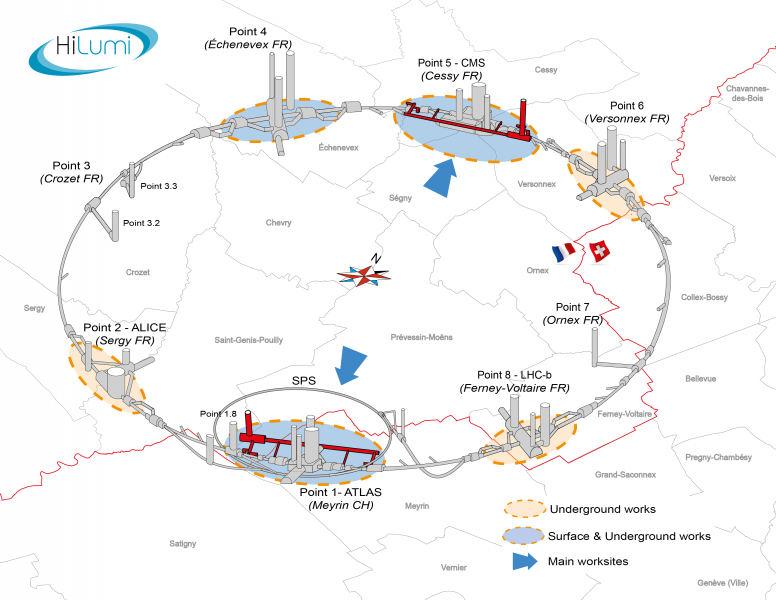
\includegraphics
						[width=\textwidth, height=.4\textheight]
						{p1-figs/hl-upgrade.png}
				 	\end{figure}

        \end{column}
        \end{columns}

        \begin{minipage}{\textwidth}
					\begin{figure}
						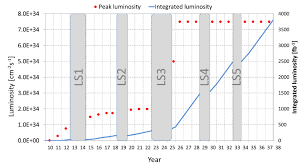
\includegraphics
						[width=\textwidth, height=.4\textheight]
						{p1-figs/hl.png}
				 	\end{figure}
        \end{minipage}  

    }

    \frame{
      \frametitle{High Luminosity LHC \& ITk Upgrades}
      %

        \begin{columns}[T,onlytextwidth]
        \begin{column}{.54\textwidth}

        \begin{block}{ $x10$ increase in instantaneous luminosity! }
            \begin{itemize}
              \item $L = $\num{1e73} fb$^{-1}$ s$^{-1} \rightarrow 
                     L = $ \num{1e74} fb$^{-1}$ s$^{-1} $ \\
              \item More particles, more problems
            \end{itemize}
          \end{block}

        \end{column}
        \begin{column}{.4\textwidth}
				\vspace{-0.5cm}
					\begin{figure}
						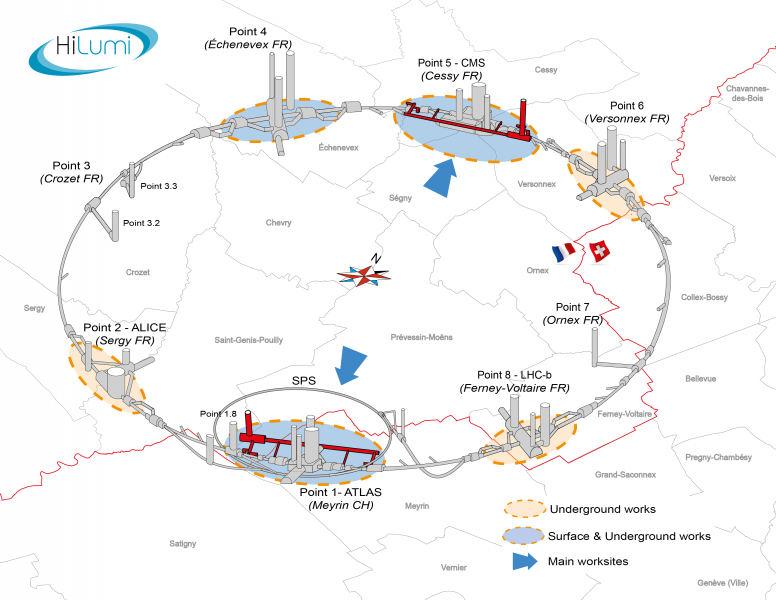
\includegraphics
						[width=\textwidth, height=.4\textheight]
						{p1-figs/hl-upgrade.png}
				 	\end{figure}

        \end{column}
        \end{columns}

        \begin{minipage}{\textwidth}
          \begin{block}{ The inner detector has insufficient:}
            \begin{itemize}
                \item radiation hardness
                \item granularity
                \item bandwidth
            \end{itemize}
          \end{block}
        \end{minipage}  

    }
   
    % ============================================================== %
    %
    % Our Progress
    %
    % ============================================================== %
    
    \section{Our Progress}
    
    \frame{
        \frametitle{ATLYS Board}
        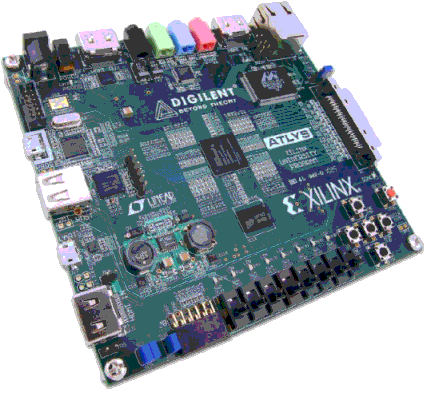
\includegraphics[width=0.5\paperwidth]{images/atlys_pic.png}
    }
    
    \frame{
        \frametitle{Obstacles}
        fuck
    }

    % ============================================================== %
    %
    % Acknowledgements
    %
    % ============================================================== %
    
    \section{Acknowledgements}
    

    \frame{
        \frametitle{Acknowledgements}
        We would like to acknowledge the University of Michigan Department of Physics, specifically Jean Krisch, Tom Schwarz, and Steven Goldfarb. 

        We would also like to acknowledge the support of the Lounsbery foundation.   \\
        %More content goes here
      \begin{tikzpicture}[remember picture, overlay]
        \node[anchor=south west, %anchor is bottom left corner of the graphic
              xshift=2.4cm, %shifting around
              yshift=0.4cm]
       at (current page.south west) %left bottom corner of the page
        { 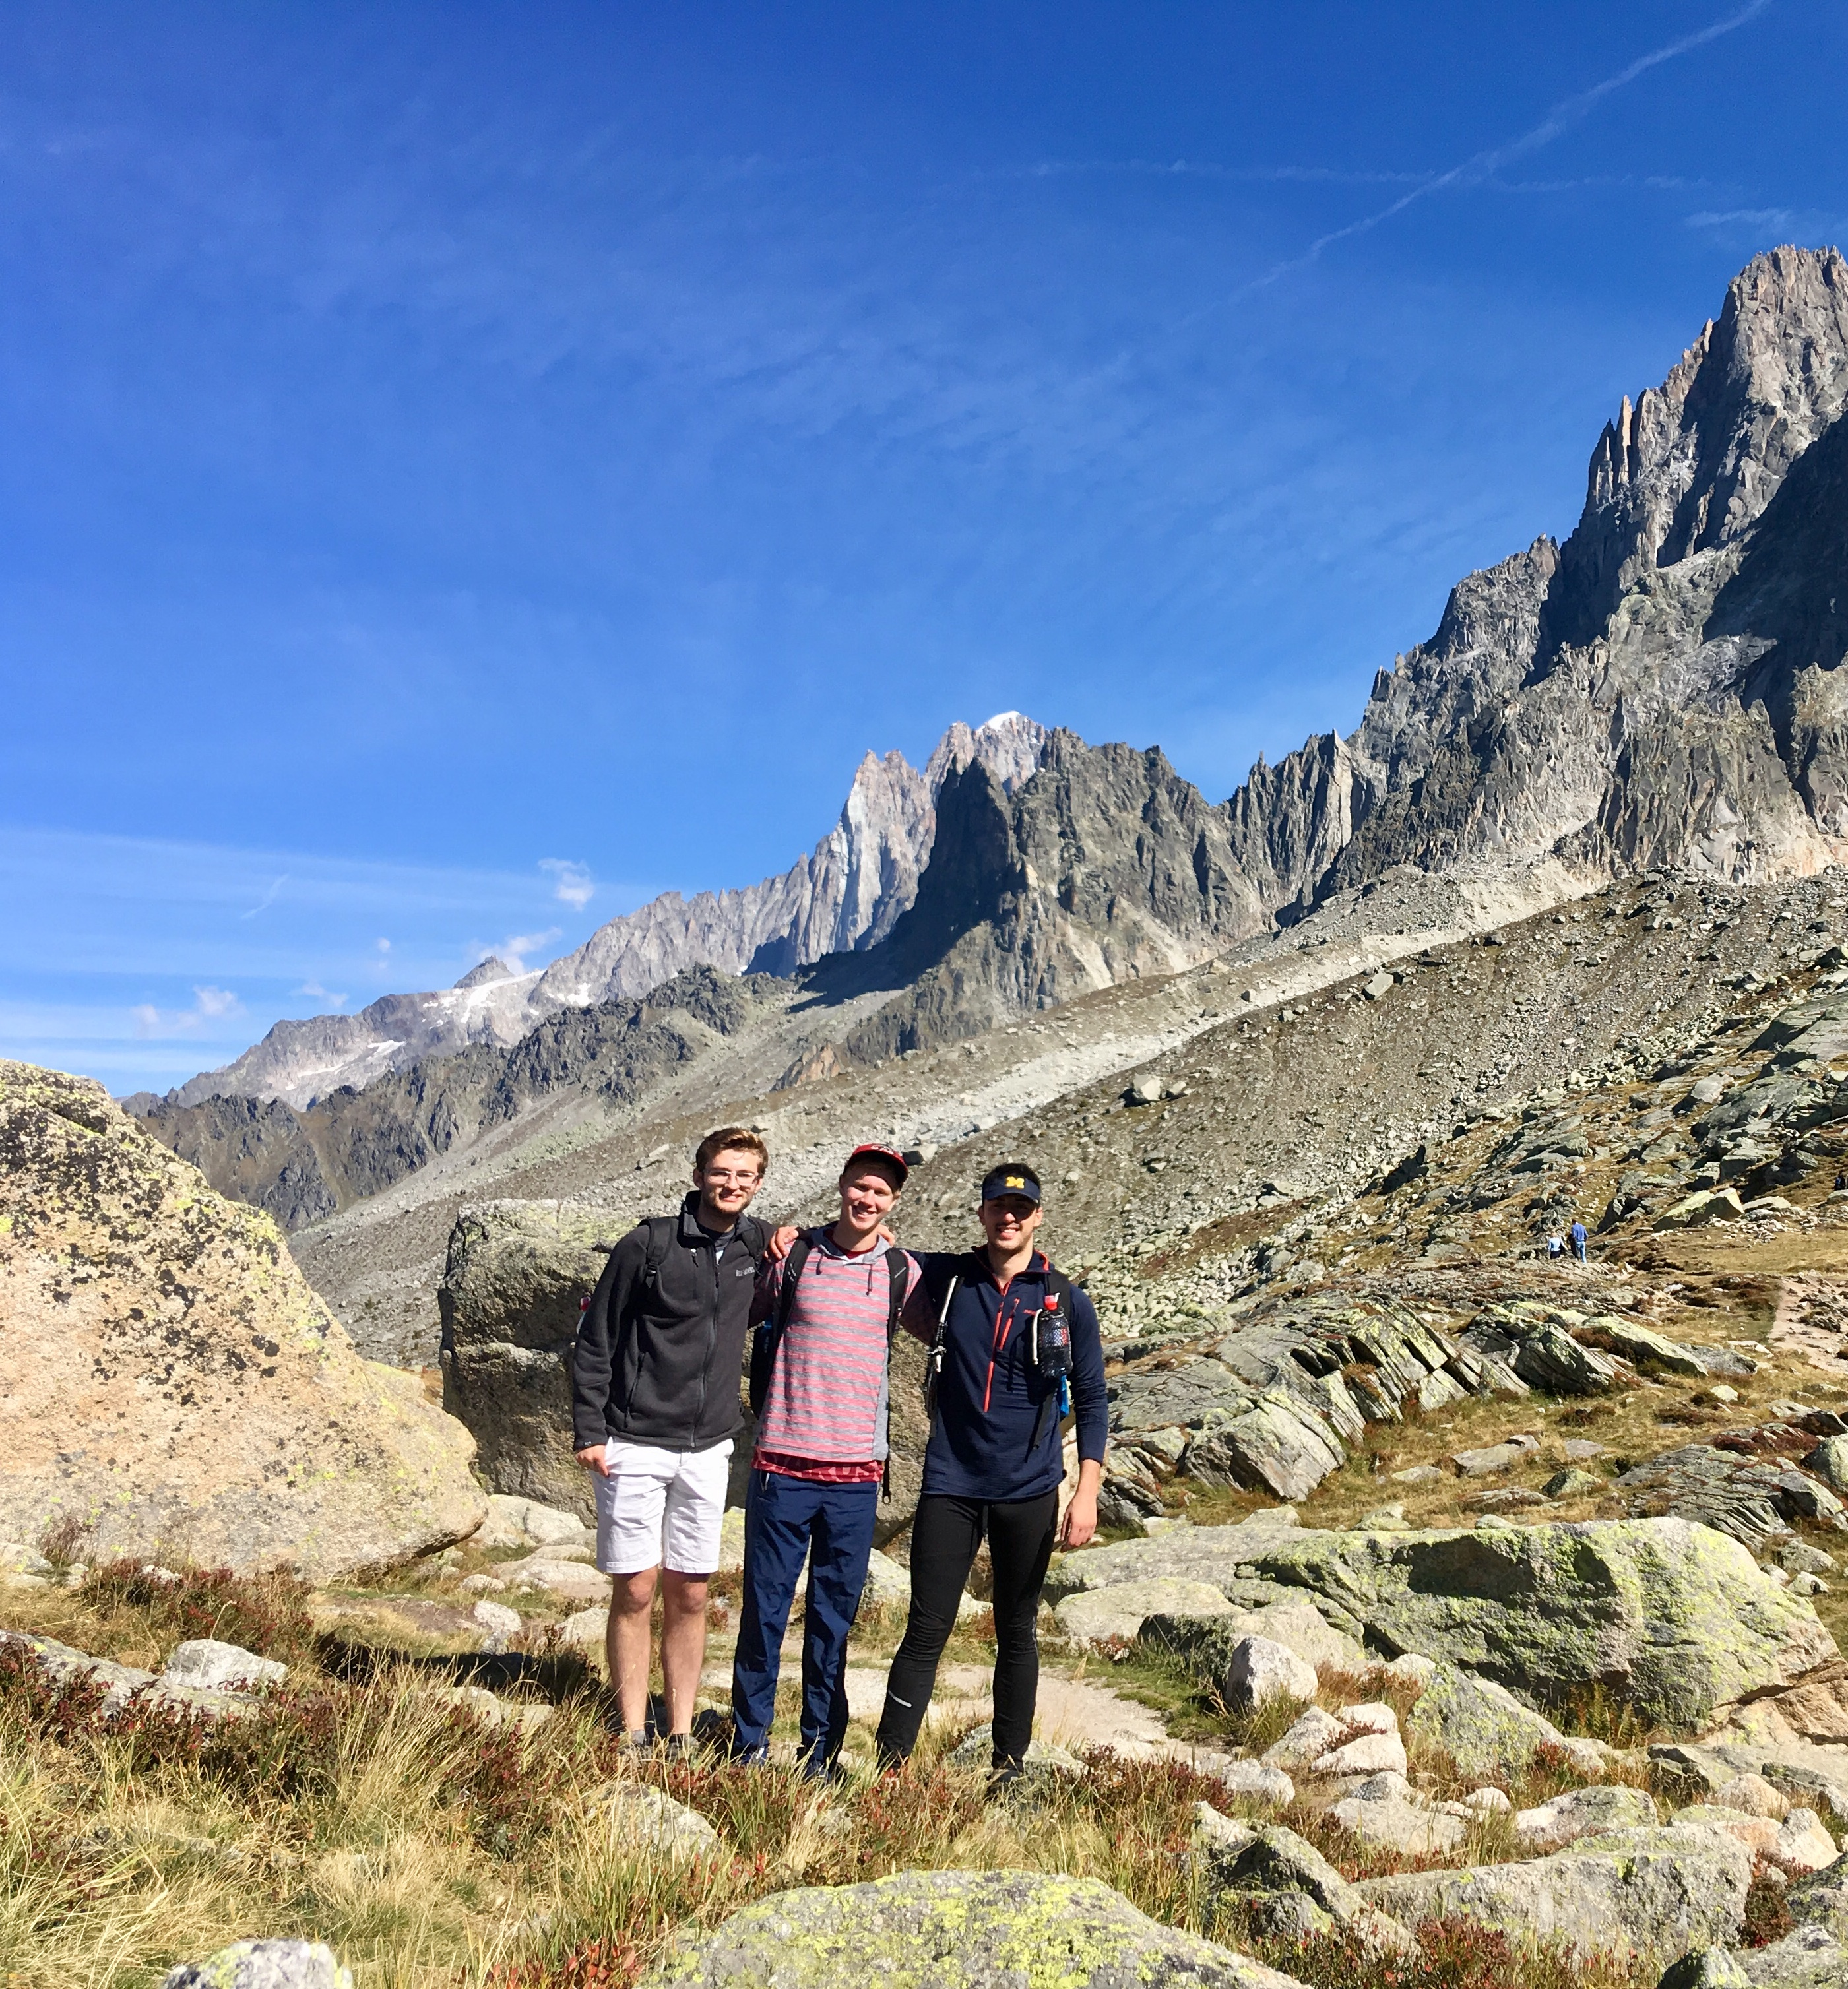
\includegraphics[scale=0.05,trim={0 0 0 35cm },clip]
        {p1-figs/cham.jpg} };

        \node[anchor=south east, %anchor is bottom left corner of the graphic
              xshift=-2.4cm, %shifting around
              yshift=0.4cm]
       at (current page.south east) %left bottom corner of the page
        {	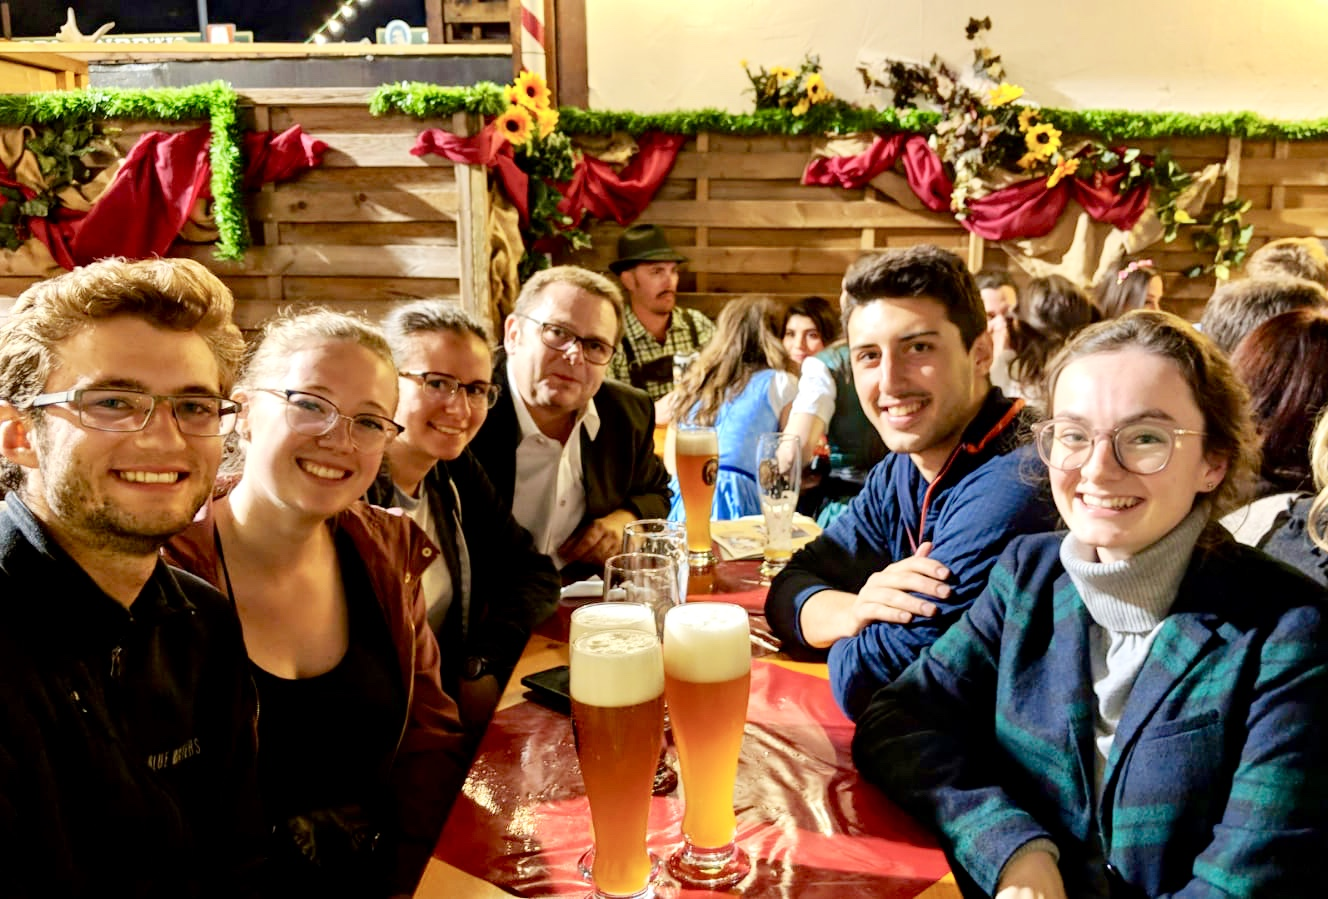
\includegraphics[width=0.33\paperwidth]{p1-figs/okto.jpg} };
			\end{tikzpicture}


    }

    \section{}
    \cernSplashWhite

\end{document}
